\message{ !name(paper.tex)}\documentclass[10pt,twocolumn,letterpaper]{article}

\usepackage{cvpr} \usepackage{times} \usepackage{epsfig}
\usepackage{graphicx} \usepackage{amsmath} \usepackage{amssymb}
\usepackage{subfig}

% Include other packages here, before hyperref.

% If you comment hyperref and then uncomment it, you should delete
% egpaper.aux before re-running latex.  (Or just hit 'q' on the first
% latex run, let it finish, and you should be clear).
\usepackage[pagebackref=true,breaklinks=true,letterpaper=true,colorlinks,bookmarks=false]{hyperref}


% \cvprfinalcopy % *** Uncomment this line for the final submission

\def\cvprPaperID{84} % *** Enter the 3DIMPVT Paper ID here
\def\httilde{\mbox{\tt\raisebox{-.5ex}{\symbol{126}}}}

% Pages are numbered in submission mode, and unnumbered in
% camera-ready
\ifcvprfinal\pagestyle{empty}\fi
\begin{document}

\message{ !name(paper.tex) !offset(705) }
\begin{figure*}
  \centering
  \subfloat[][]{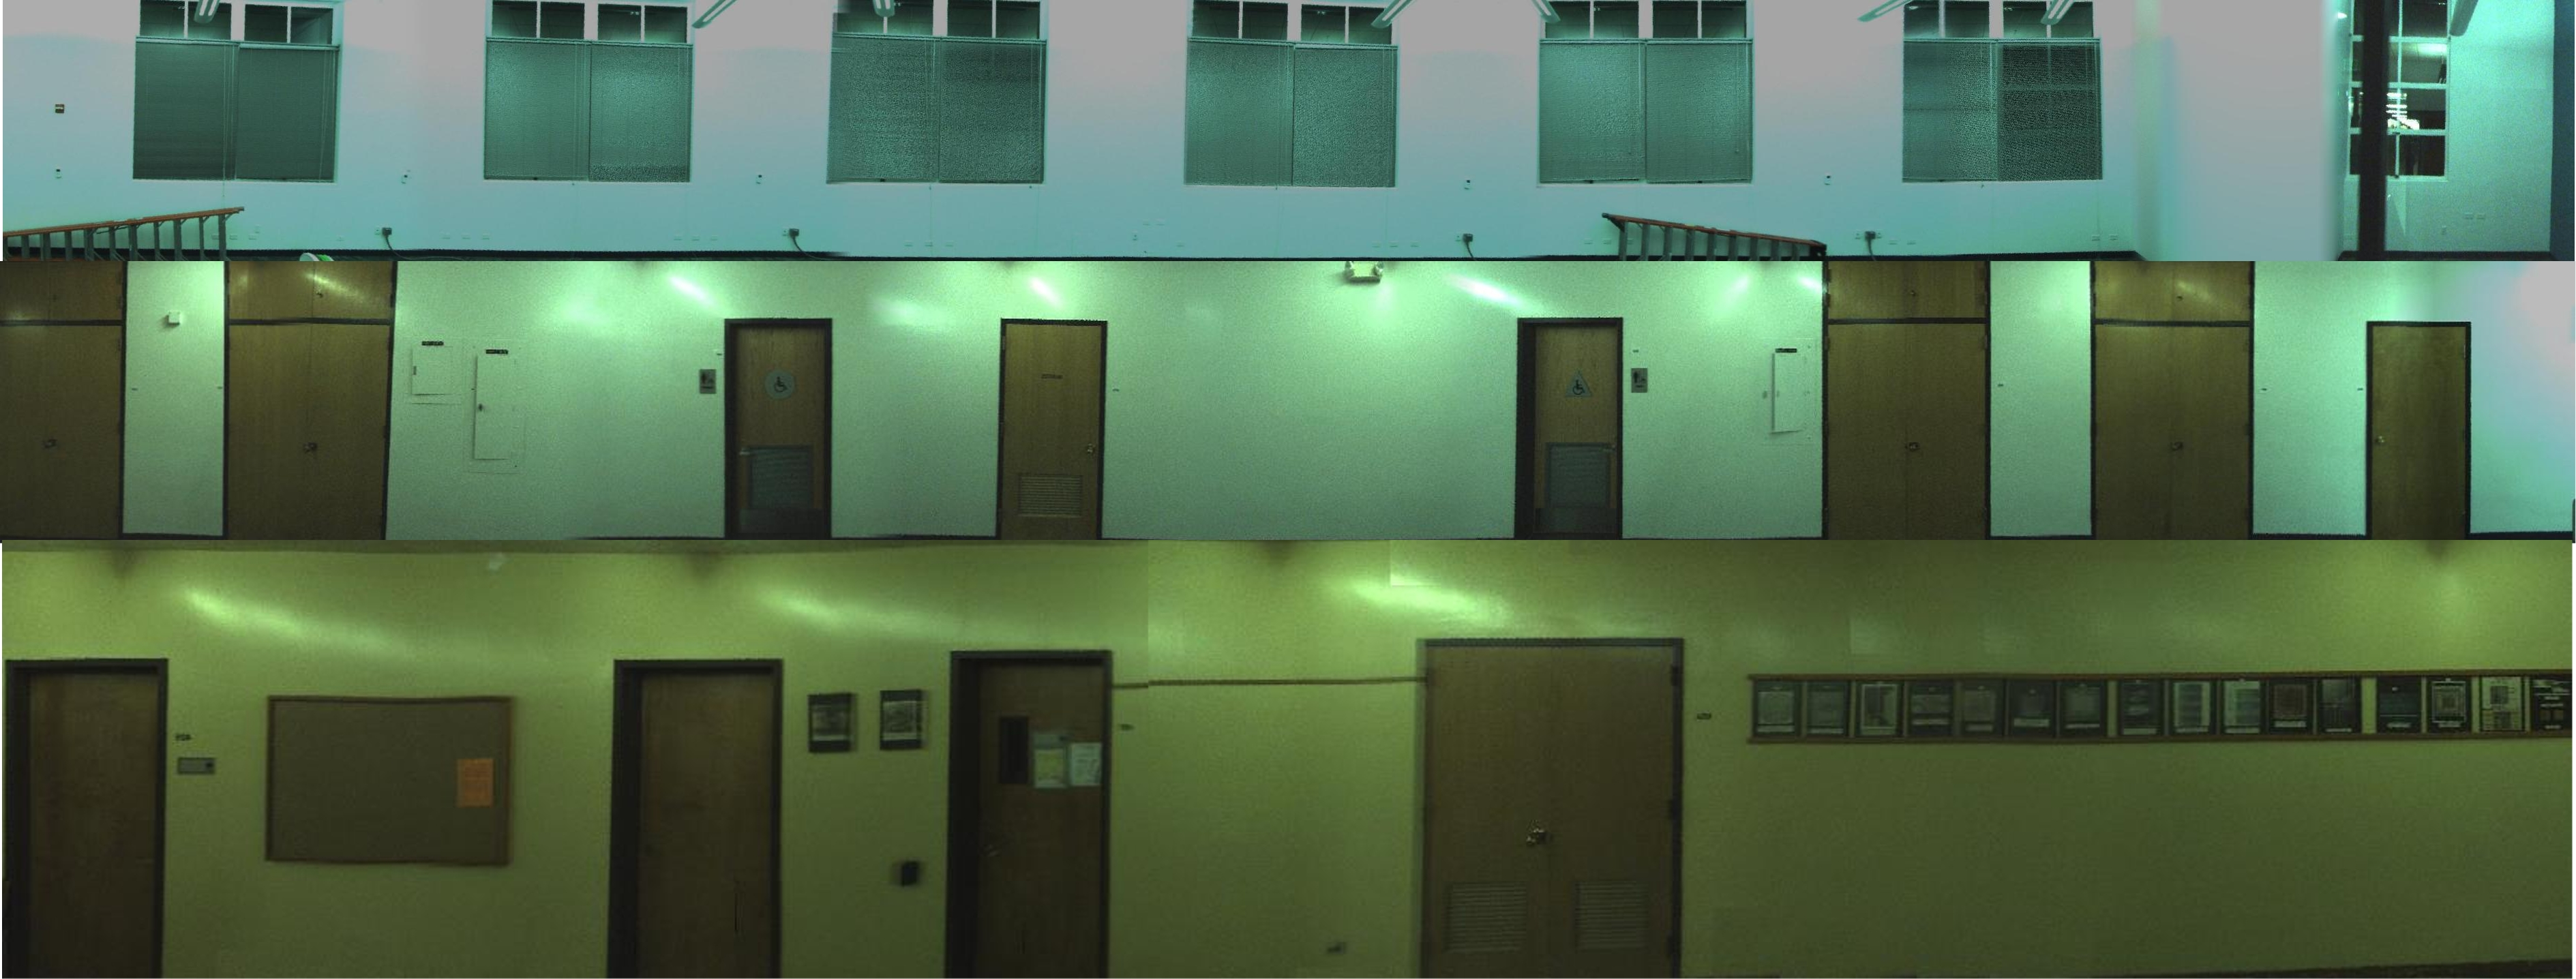
\includegraphics[width=3in]{finalfloors.jpg}}
  ~~~
  \centering
  \subfloat[][]{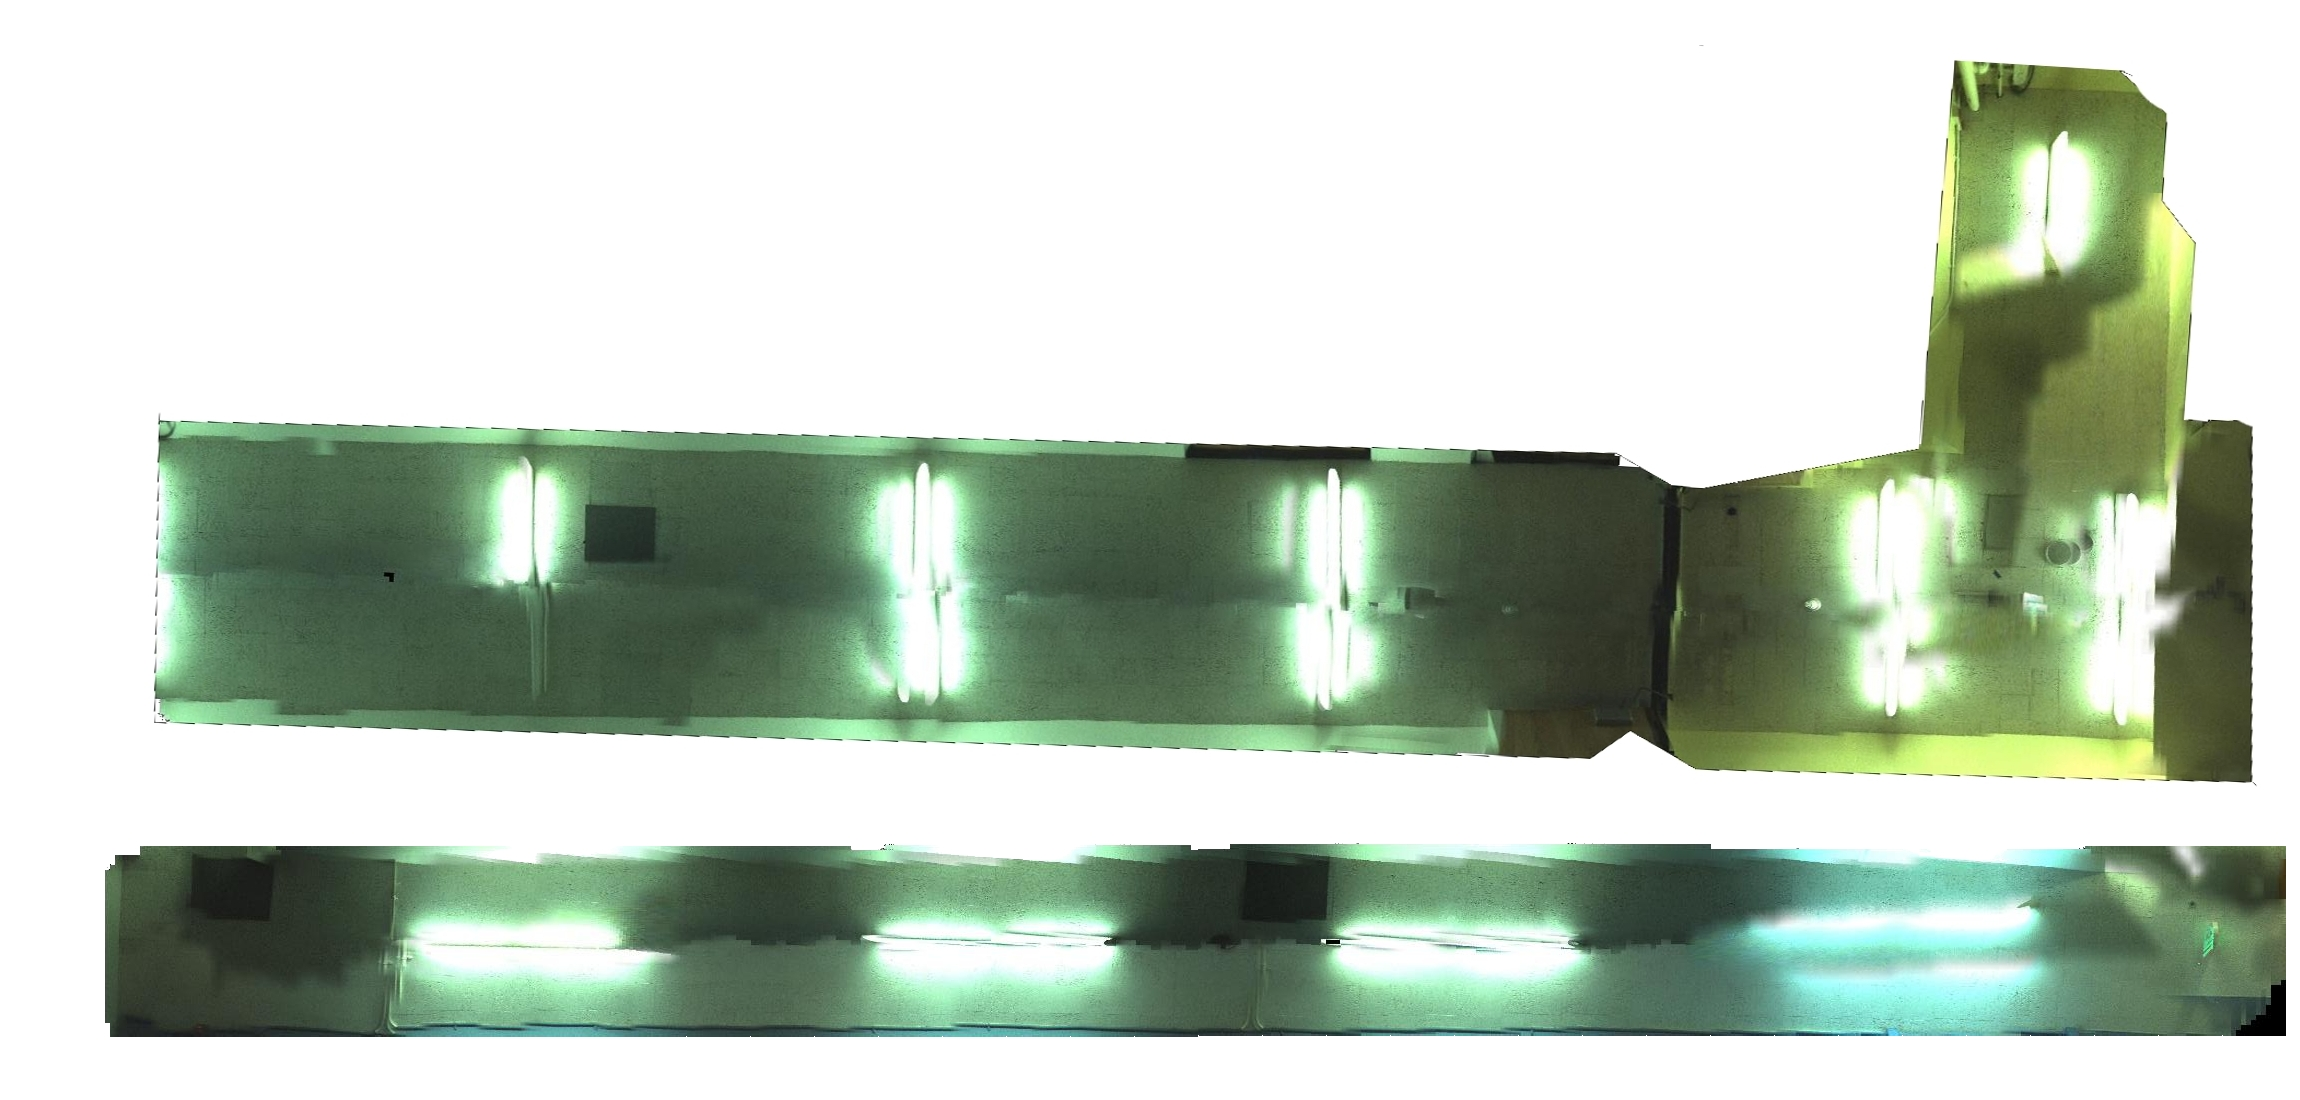
\includegraphics[width=3in]{finalceilings.jpg}}

  \centering
  \subfloat[][]{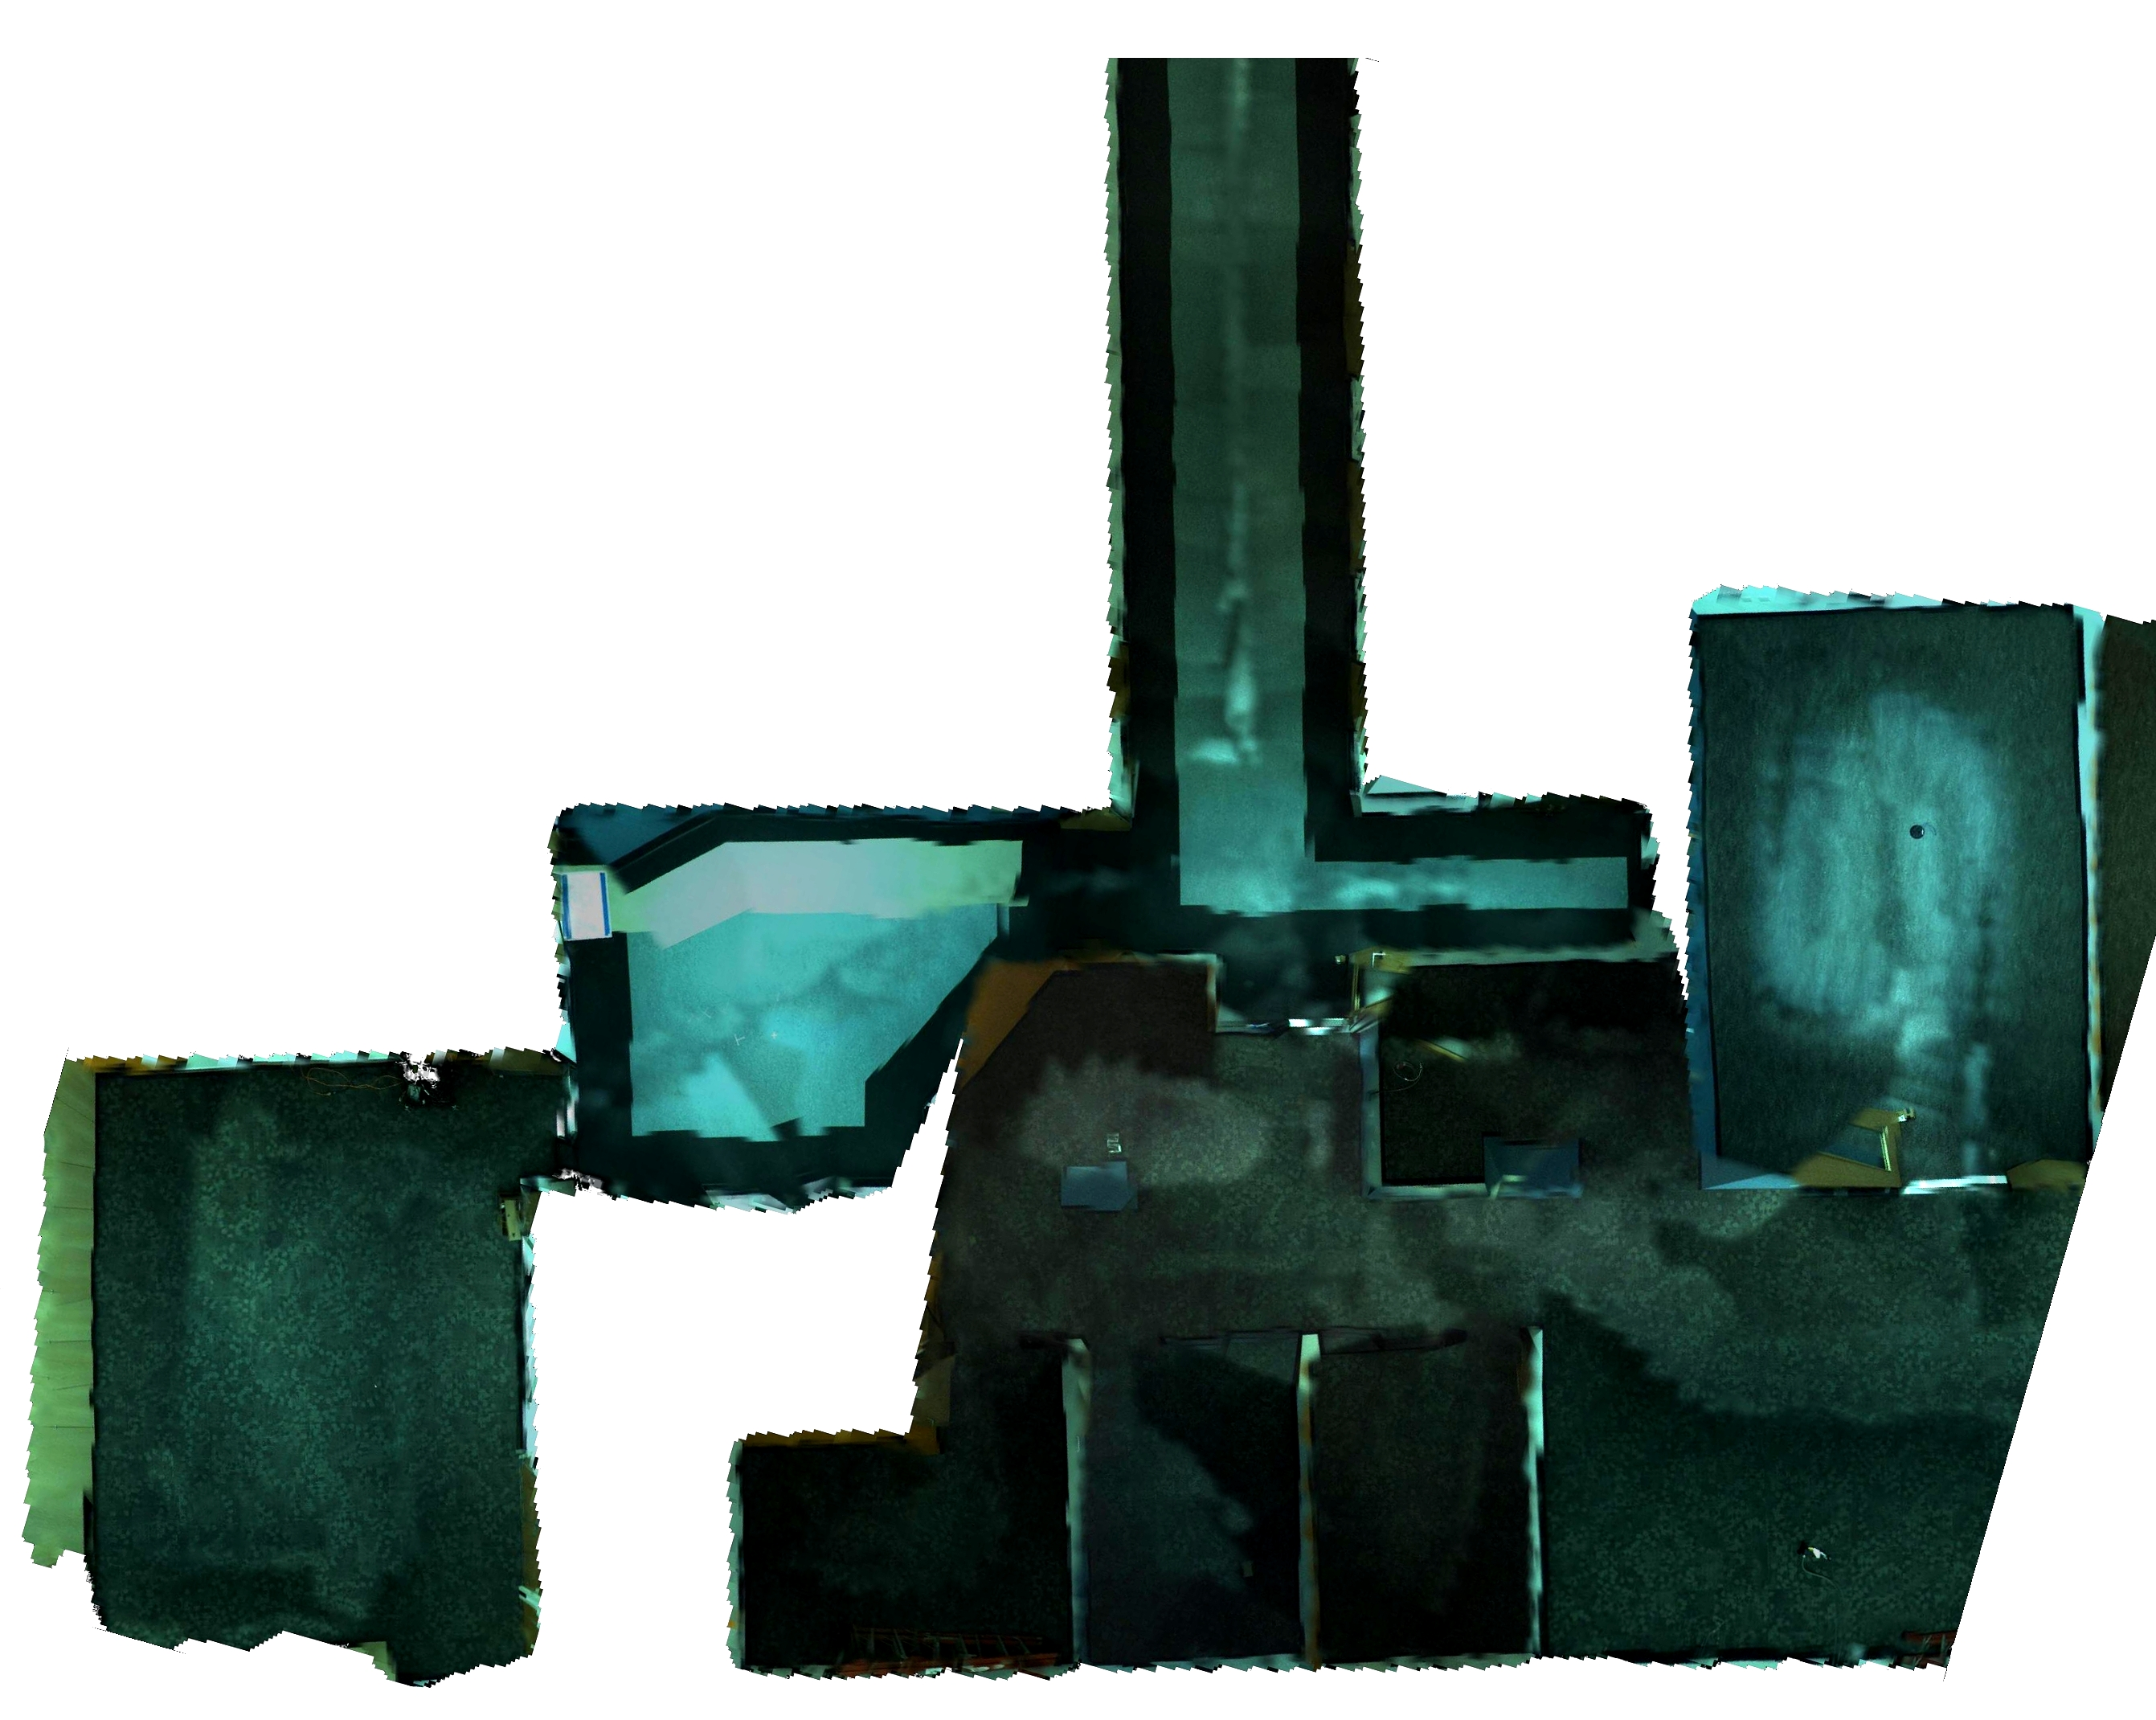
\includegraphics[height=2in, width=3in]{floorcropped.jpg}}
  ~~~
  \centering \subfloat[][]{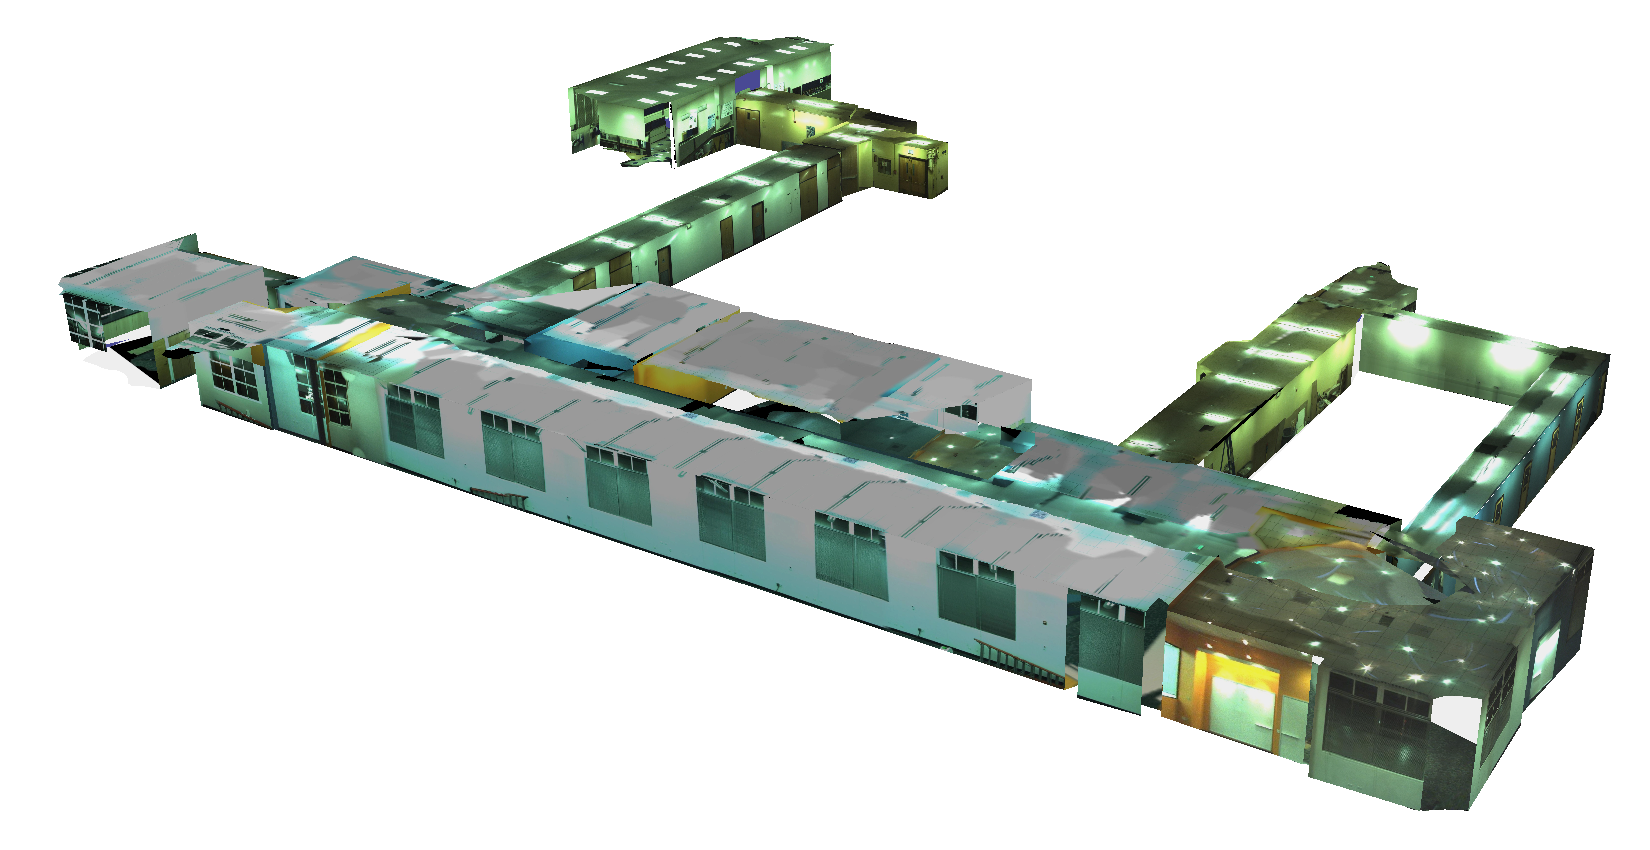
\includegraphics[width=3in]{fullmodel.png}}
  \caption{Examples of our final texture mapping output for (a) walls,
    (b) ceilings, (c) an entire floor, (d) a full model.}
  \label{fig:results}
\end{figure*}
\message{ !name(paper.tex) !offset(708) }

\end{document}
